\documentclass[12pt, letterpaper]{article}
\usepackage[utf8]{inputenc}
\usepackage{calc} 
\usepackage[spanish]{babel}
\usepackage[utf8]{inputenc}
\usepackage{graphicx} 
\usepackage[left=2.58cm, right=2.58cm, tmargin=2cm, bmargin=2cm]{geometry} 
\usepackage{url,hyperref}

\title{Practica1}
\author{Equipo}
\date{\today}

\begin{document}
    \begin{minipage}{2cm}
		\centering
		
\includegraphics[width=2cm]{ipn-logo.png}

	\end{minipage}
	\hfill 
	\begin{minipage}{\linewidth-6cm}
		\centering
        \huge
		\textsc{Instituto Politécnico Nacional}
	\end{minipage}
	\hfill 
	\begin{minipage}{3cm}
		\centering
		
\includegraphics[width=3cm]{upiita-logo.png}
	\end{minipage}
	
	\vspace{0.8cm}
	
	\begin{center}
		\Large
		\textsc{Unidad Profesional Interdisciplinaria de Ingeniería y Tecnologías Avanzadas}
		
		\vspace{1.2cm}
		\huge
		\textsc{Práctica 1}
		
	
	\vspace{1.2cm}
	
		\large
		Profesor\\
		\vspace{0.3cm}
		\large
		\textbf{Iliac Huerta Trujillo}
		
		\vspace{1.2cm}
		\large
		Unidad de Aprendizaje \\
		\vspace{0.3cm}
		\large
		\textbf{Programación Orientada a Objetos}
	
		\vspace{1.2cm}
		\large
		\textbf{Presenta}\\
		\vspace{0.3cm}

    \begin{table}[h]

        \centering
        \large
        \begin{tabular}{lr}
            Ramírez López Emilio & 2022640230  \\
            Sánchez Díaz Nadya & 2022640236 \\
            Velázquez Osorio Samara Ishtar & 2022640188 \\
        \end{tabular}

    \end{table}
	
		\vspace{1.2cm}
		20 de septiembre de 2022
		
	\end{center}
	
    \newpage
    
    \tableofcontents
    \listoffigures
    \newpage
    
    \section{Planteamiento del problema}
    Un almacén de pedidos por correo cuenta con 5 productos distintos en inventario identificados como producto 1, producto 2, producto 3, producto 4 y producto 5. De los cuales sus respectivos precios son \$2.98, \$4.50, \$9.98, \$4.49 y \$5.58.
    
    
    Se busca un método eficiente para calcular la cantidad de productos vendidos y el total de ingresos por venta y al final del día, al cierre. 
    
    
    \section{Justificación}
    Un programa de este tipo puede ser de mucha utilidad como base para el sistema de diferentes negocios y así tener un control y registro de las ventas realizadas día a día, haciendo de este un proceso más eficiente al llevarlo a cabo de forma automática.
    
    Además, resulta un ejercicio útil para familiarizarnos con estructuras tales como do-while y switch.
 

    
    
    \section{Propuesta de solución}
   Creamos un programa que funcione como registro de las compras que se realizan por medio de los datos que se reciben. Cuando el usuario señale que ya no requiere de más productos, se le imprimirá un recibo que marque cuántos productos se compraron y cuánto es el total de la venta. Al finalizar las ventas, estas se irán sumando para que, cuando se solicite el cierre de ventas del día, se imprima el registro de la cantidad total vendida de cada producto y el valor total de la venta del día.
   
   El programa lee una serie de números que se introducen consecutivamente para poder conocer:
   \begin{enumerate}
       \item El número del producto
       \item La cantidad del producto
   \end{enumerate}
   
    
    \section{Análisis y diseño}
      Al analizar el problema podemos ver que necesitamos usar la estructura switch para controlar el precio total de cada producto que se vende y también el uso de do-while para realizar la primera venta y seguir repitiendo hasta que se nos pida cerrar la cuenta actual y también la cuenta al final del día. Cada case en el switch será un producto diferente y nos permitirá calcular la suma del costo total de la venta.
      
      A continuación se presentan diagramas que ayudarán a comprender de manera gráfica nuestra propuesta de solución.
         \begin{enumerate}
            \item \textit{Diagrama de actividades:} Es un tipo de diagrama dentro del lenguaje unificado de modelado (UML). El cual nos permitirá visualizar de manera general el flujo de actividades dentro de nuestro programa.
            \item \textit{Diagrama de flujo:} Representa la esquematización gráfica de un algoritmo, el cual muestra los pasos a seguir para la solución de un problema.
        \end{enumerate}
        
    \newpage
      
    \begin{figure}[h]
    \centering
    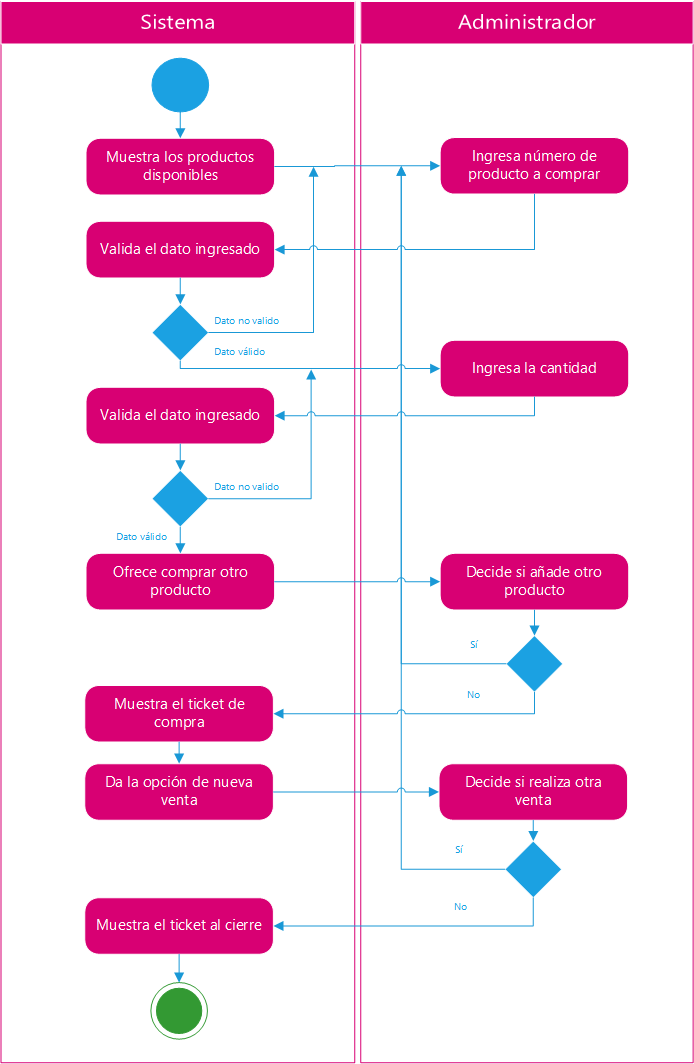
\includegraphics[scale=0.785]{D-actividades-p1.png}
    \caption {Diagrama de actividades \label{fig:Fig1}}
    \end{figure}
    
   
     \begin{figure}[p]
    \centering
    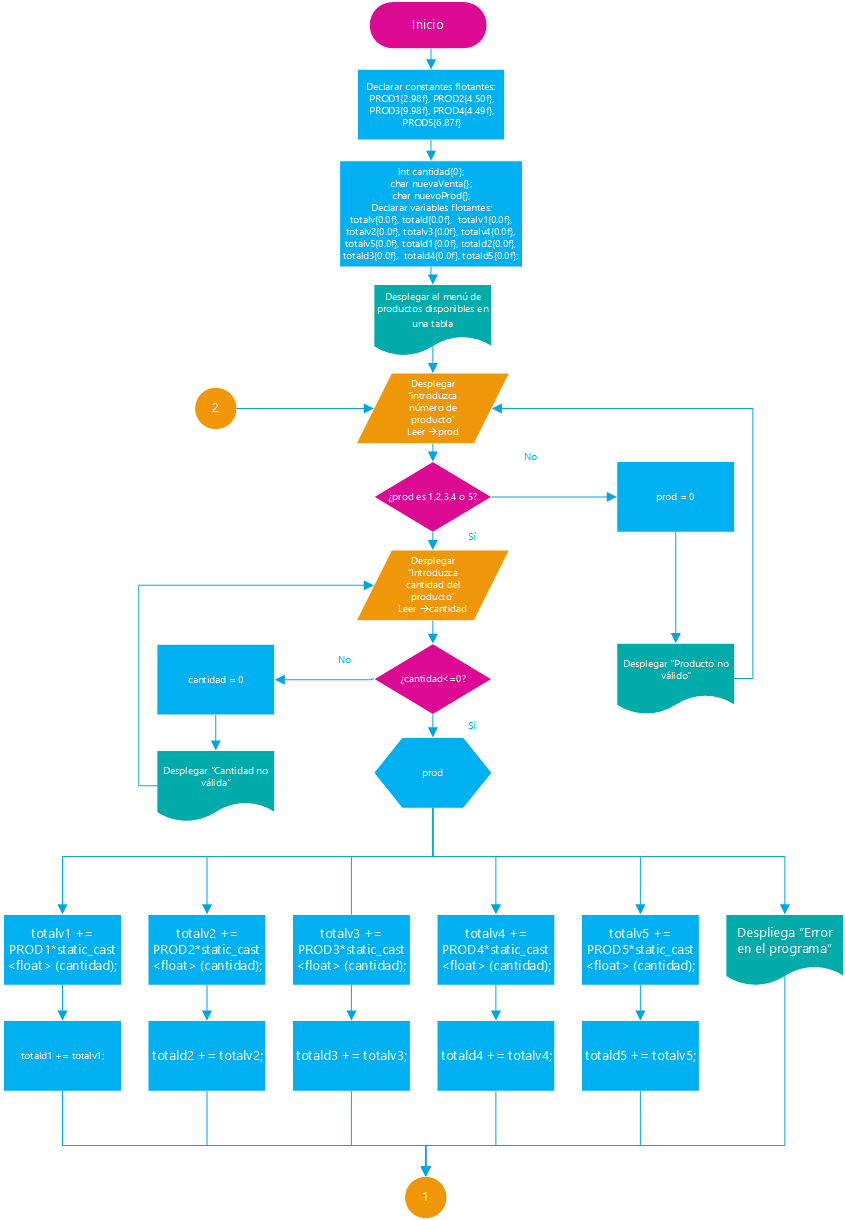
\includegraphics[width=15cm]{D-flujo-p1.png}
    \caption {Diagrama de flujo \label{fig:Fig2}}
    \end{figure} 
    
     \begin{figure}[p]
    \centering
    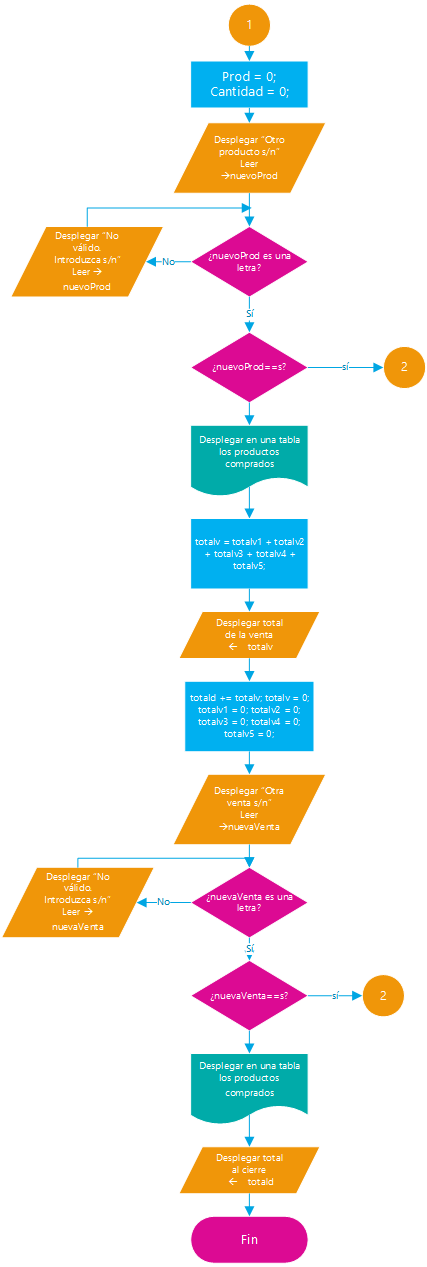
\includegraphics[width=7.5cm]{D-flujo2-p1.png}
    \caption {Diagrama de flujo \emph{continuación} \label{fig:Fig3}}
    \end{figure} 
    
    
    \newpage
     
    \section{Desarrollo e implementación}
    
    \subsection{Desarrollo del programa}
    En el programa, comenzamos declarando como constantes de tipo flotante los precios de cada producto.
    
    \begin{figure}[h]
    \centering
    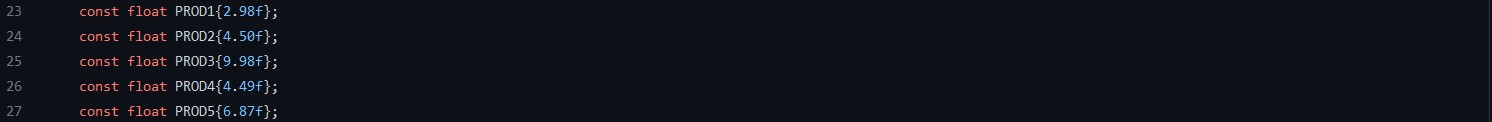
\includegraphics[width=16cm]{constantes.jpg}
    \caption {Constantes \label{fig:Fig4}}
    \end{figure}

    \vspace{0.8cm}
    
    Seguida de variables de tipo entero para almacenar el número de producto y su cantidad, variables de tipo caracter para dar la opción de continuar con las ventas o no, y variables de tipo flotante para ir almacenando el total de ingresos de cada producto y total por venta y día. 
    
    \begin{figure}[h]
    \centering
    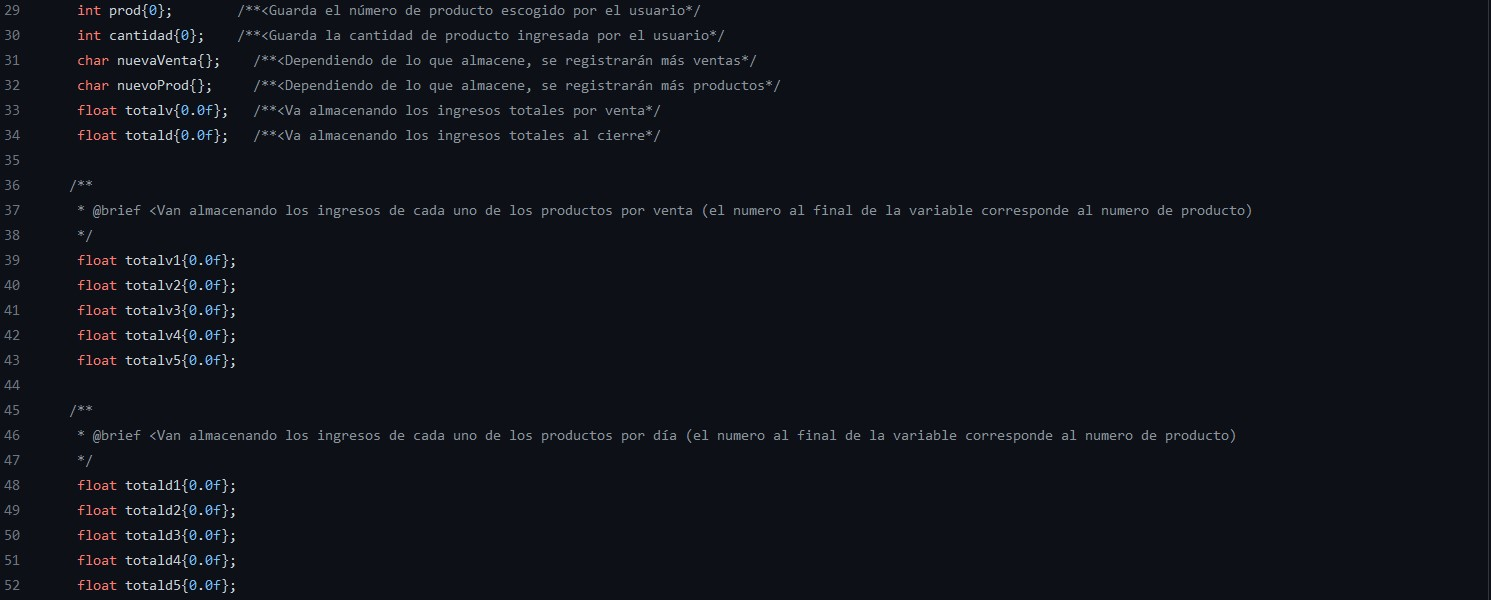
\includegraphics[width=16cm]{variables.jpg}
    \caption {Variables \label{fig:Fig5}}
    \end{figure}
    
    \vspace{0.8cm}
    
    Decidimos agregar una tabla donde se muestren los productos disponibles y su precio correspondiente para facilitar al usuario el uso del programa.
    
    \begin{figure}[h]
    \centering
    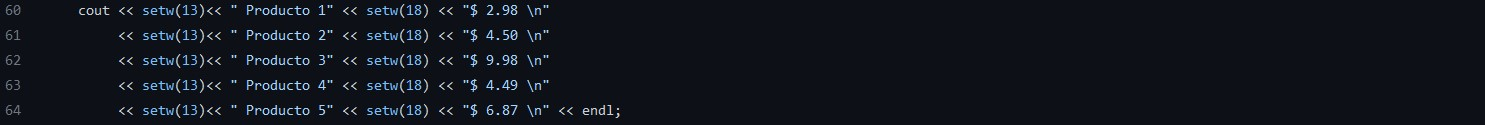
\includegraphics[width=16cm]{tabla.jpg}
    \caption {Inventario \label{fig:Fig6}}
    \end{figure}
    
    \vspace{0.8cm}
    
    Usamos un ciclo do-while para realizar al menos una venta y tener la posibilidad de continuar con otra siempre que el usuario así lo desee (que ingrese una 's'), de otra forma se dará por finalizado el día.
    
    Dentro de este ciclo tenemos otro do-while que permitirá seleccionar un producto y la cantidad deseada, dando la opción a seguir añadiendo productos siempre que el usuario ingrese una 's', de lo contrario, se cerraría la venta.
    
    Para esto, necesitamos que el usuario ingrese un número valido con el que se identifica un producto existente, para ello usamos un ciclo while, en el que se solicita al usuario ingresar el número de producto, con la condición de que prod sea igual a cero, debido a que prod se inicializó con cero, se ejecutará inicialmente y prod solo cambiará si el usuario introduce un número de tipo entero. Dentro de este while agregamos un if para asegurarse de que en caso de que se ingrese un número entero, este sea únicamente 1, 2, 3, 4 o 5.
    
    \begin{figure}[h]
    \centering
    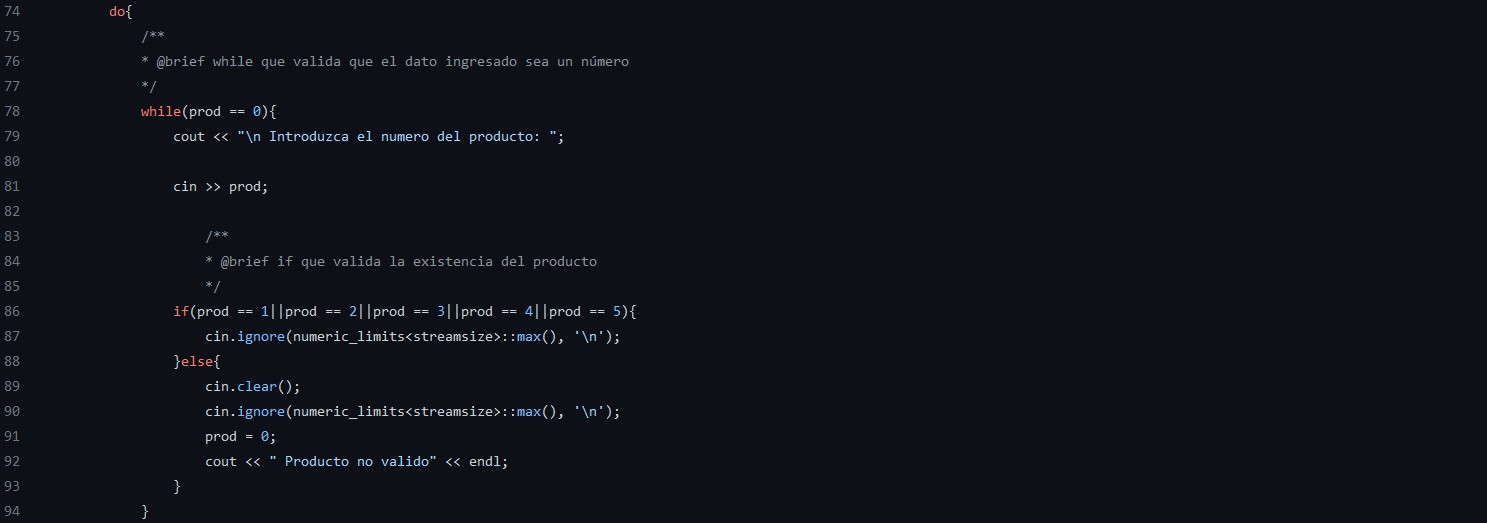
\includegraphics[width=16cm]{validacion-producto.jpg}
    \caption {Validación de producto \label{fig:Fig7}}
    \end{figure}
    
    \vspace{0.8cm}
    
    Hicimos una validación similar al momento de solicitar la cantidad del producto seleccionado, con la única diferencia de que la condición del if (que muestra el mensaje de error) es que la cantidad sea un número menor o igual a cero.
    
    \begin{figure}[h]
    \centering
    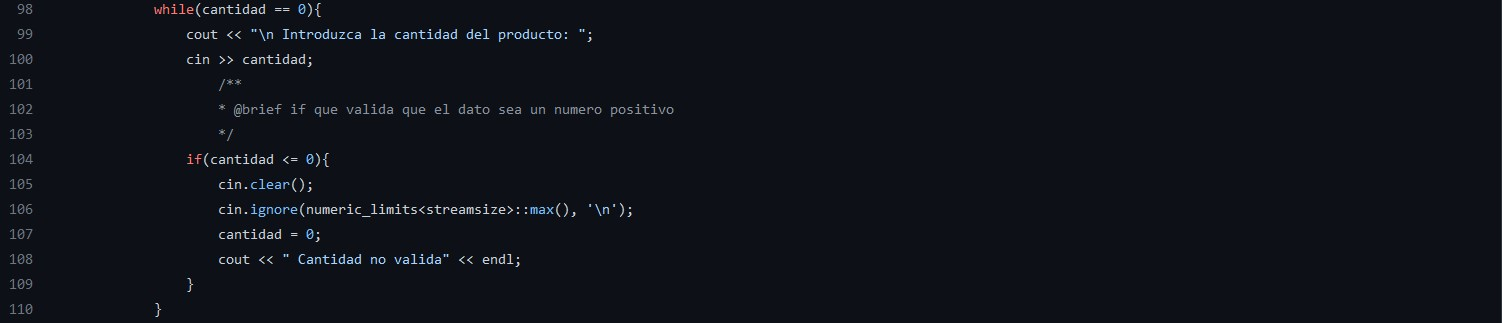
\includegraphics[width=16cm]{validacion-cantidad.jpg}
    \caption {Validación de cantidad \label{fig:Fig8}}
    \end{figure}

    \vspace{0.8cm}
    
    Una vez validado el producto y su cantidad, usamos un switch en el que cada producto representa un caso distinto, y según sea el caso hará lo siguiente:
    \begin{enumerate}
       \item Multiplicará el precio del producto por la cantidad solicitada y se acumulará en el total por venta de dicho producto.
       \item Este total por venta se irá acumulando en otra variable que representa el ingreso total del producto al cierre.
    \end{enumerate}
    
    \newpage
    
    \begin{figure}[h]
    \centering
    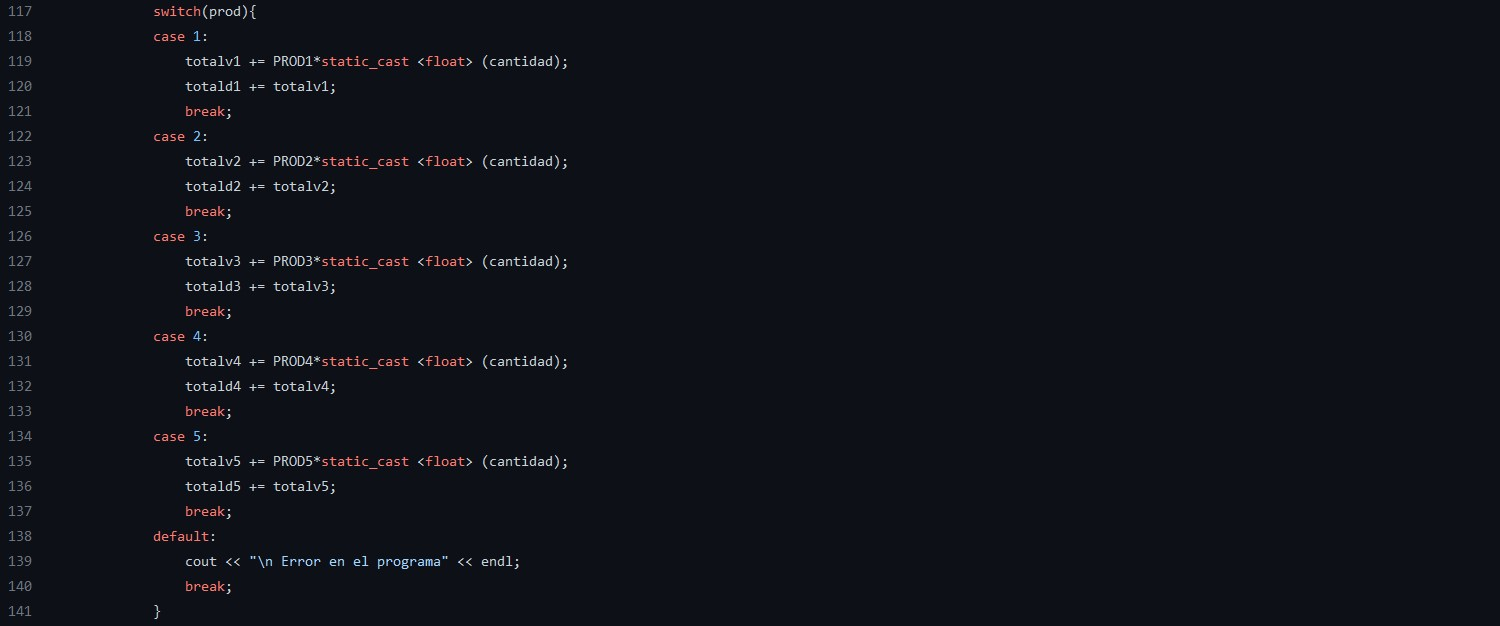
\includegraphics[width=16cm]{switch.jpg}
    \caption {Estructura switch \label{fig:Fig9}}
    \end{figure}
    
    \vspace{0.8cm}
        
    Regresamos a prod y cantidad a su valor inicial (0) para no afectar el funcionamiento de ciclos futuros en caso de que se decida agregar un nuevo producto a la venta, y para ello solicitamos al usuario ingrese 's' o 'n' según sea el caso, validando con isalpha que sea un caracter y usando tolower para que no haya diferencia entre mayúsculas y minúsuculas. 
    
    \begin{figure}[h]
    \centering
    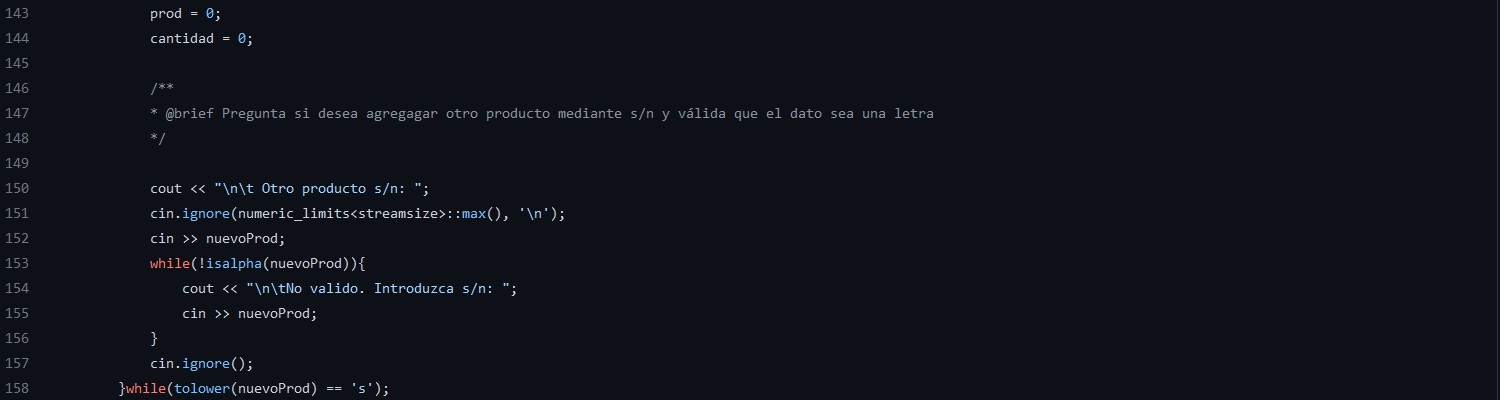
\includegraphics[width=16cm]{nuevo-prod.jpg}
    \caption {Condición del do-while interno \label{fig:Fig10}}
    \end{figure}
    
    \vspace{0.8cm}
    
    Si se eligió terminar la venta, se despliega en pantalla una tabla a modo de ticket en el que se muestra el producto vendido, la cantidad, el monto de cada producto y abajo el monto total de la venta.
    
    \newpage    
    
    \begin{figure}[h]
    \centering
    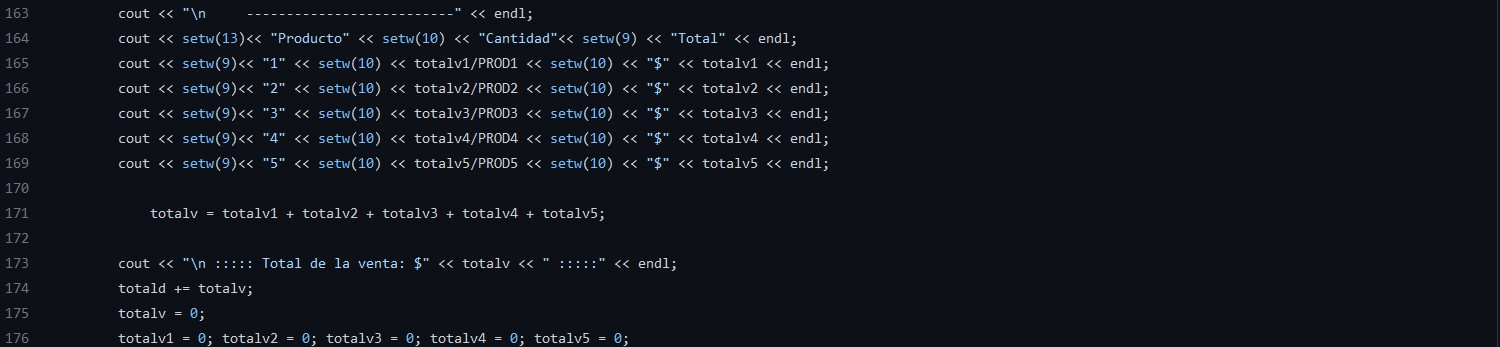
\includegraphics[width=16cm]{ticket1.jpg}
    \caption {Ticket de venta \label{fig:Fig11}}
    \end{figure}

    \vspace{0.8cm}
    
    Usando la misma lógica, se da la opción al usuario de realizar una nueva venta y se valida el dato ingresado de la misma forma. De no haber elegido 's' salimos del ciclo do-while y se imprime una tabla similar a la de cada venta con la diferencia de mostrar el monto acumulado en todo el día.
    
    \begin{figure}[h]
    \centering
    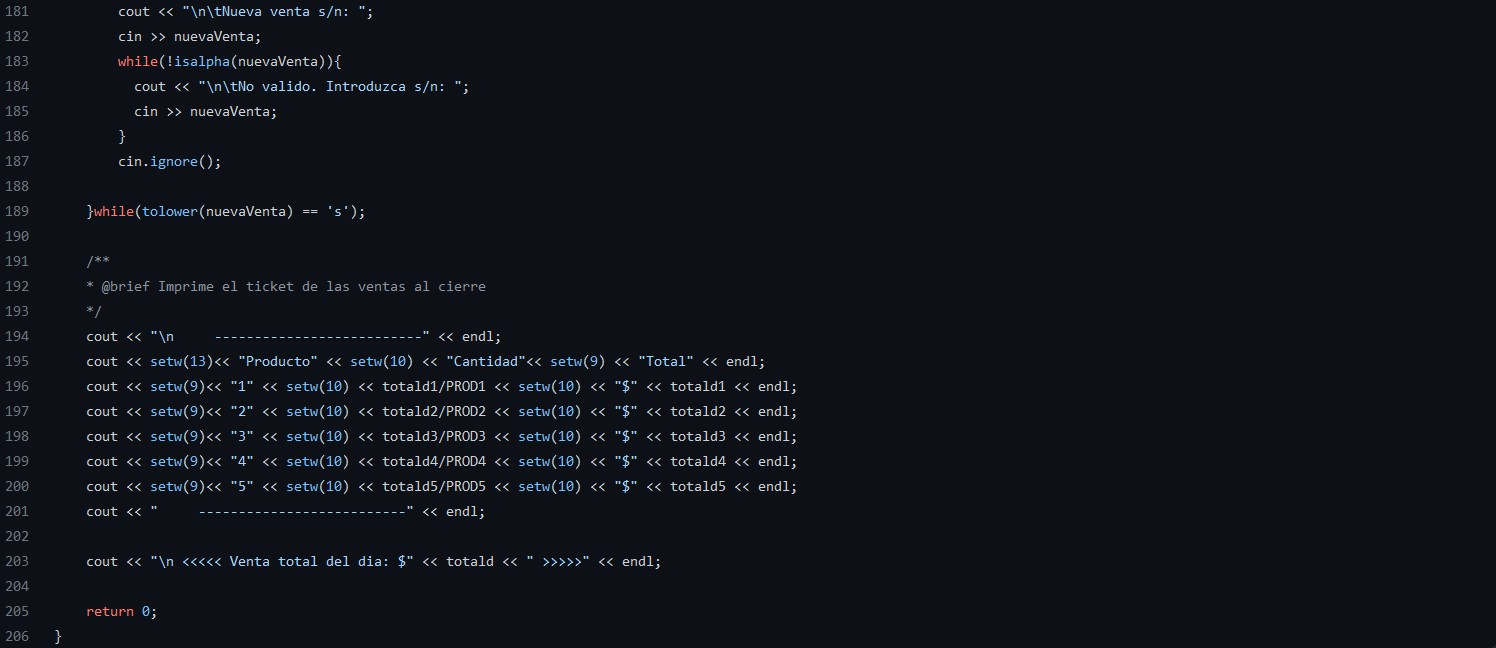
\includegraphics[width=16cm]{ticket2.jpg}
    \caption {Condición del do-while externo y ticket al cierre \label{fig:Fig12}}
    \end{figure}

    \vspace{0.8cm}
    
    \subsection{Implementación}
    Incluimos un ejemplo del funcionamiento del programa.
    El usuario hará 3 ventas:
    \begin{enumerate}
       \item En la primer venta se comprarán 2 productos: 
       \begin{enumerate}
             \item 26 unidades del producto 4.
             \item 31 unidades del producto 1.
         \end{enumerate}
         
       \item En la segunda venta se comprarán 4 productos:
       \begin{enumerate}
             \item 96 unidades del producto 5.
             \item 300 unidades del producto 2.
             \item 42 unidades del producto 4.
             \item 50 unidades del producto 3.
         \end{enumerate}
         
       \item En la tercera venta se comprará 1 producto:
       \begin{enumerate}
             \item 11 unidades del producto 3.
         \end{enumerate}
    \end{enumerate}       
    
    \vspace{1.5cm}
  
    \begin{figure}[h]
    \centering
    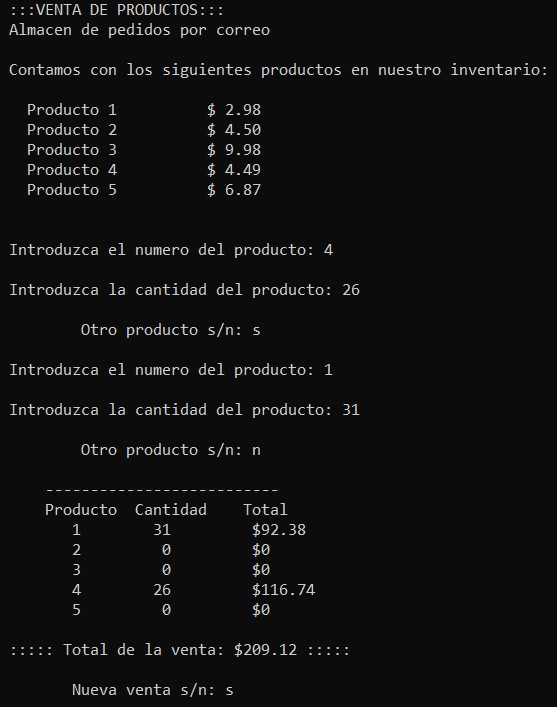
\includegraphics[width=10cm]{venta1.jpg}
    \caption {Ejemplo venta 1 \label{fig:Fig13}}
    \end{figure} 
             
    \begin{figure}[p]
    \centering
    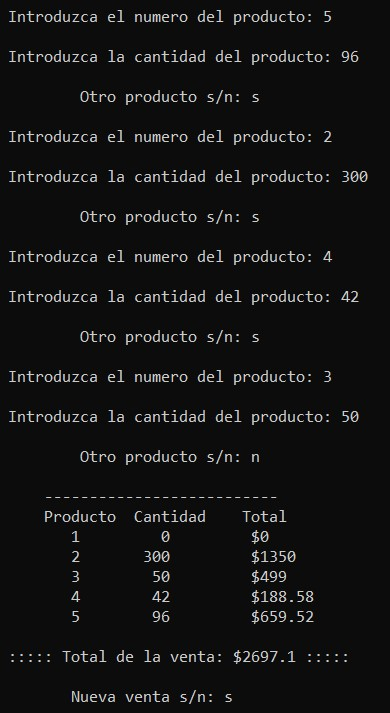
\includegraphics[width=10cm]{venta2.jpg}
    \caption {Ejemplo venta 2 \label{fig:Fig14}}
    \end{figure} 
             
    \begin{figure}[p]
    \centering
    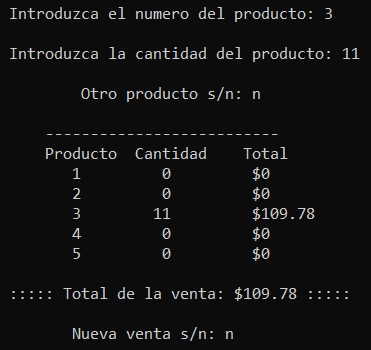
\includegraphics[width=10cm]{venta3.jpg}
    \caption {Ejemplo venta 3 \label{fig:Fig15}}
    \end{figure}
         
    \begin{figure}[p]
    \centering
    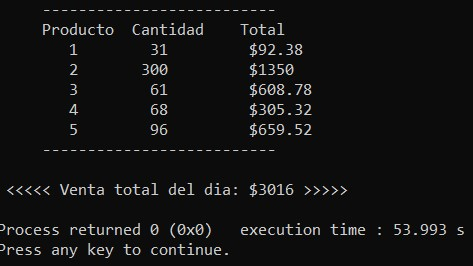
\includegraphics[width=10cm]{cierre.jpg}
    \caption {Ejemplo cierre \label{fig:Fig16}}
    \end{figure}
         
    \newpage

    \section{Conclusiones}
    En la realización de la práctica se trabajó con uno de los usos prácticos que se le puede dar a la sentencia switch asignando cada caso a un producto. Además de comprobar la utilidad del ciclo do-while al realizar iteraciones hasta que se indique que ya no se va a comprar más producto en una venta o que se finalizaron las ventas del día. De igual forma, en la validación de datos se implementaron verificadores del flujo de entrada para evitar problemas de iteraciones infinitas sin control.
    
\end{document}
